\graphicspath{{Fusion/}}

\section{Introduction}\label{sec:intro}
Thin beams of intense electron precipitation are associated with spatially discrete aurora and families of wave modes arising from the beam-destabilized plasma \citep{akbari2015}.
Incoherent scatter radar (ISR) routinely shows F-region enhancements in the ion-acoustic and plasma line spectra associated with wave mode destabilization due to this intense precipitation \citep{schlatter2014}.
Optical measurements of finely structured prompt auroral emissions are strongly correlated with incoherent scatter radar (ISR) backscatter power \citep{sullivan2008,michell2009,michell2014}.
Fast-sampling auroral tomography systems can estimate particle precipitation differential number flux as a function of space, energy and time based on prompt auroral emissions \citep{hirsch2016}.
It is often difficult to determine the direct mechanism by which the energy of the precipitating particles is transformed into free energy for plasma waves.
The exact mechanism underlying the intensification of ion-acoustic waves regularly observed by ISRs in the form of strong backscattered echoes called NEIALs (Naturally Enhanced Ion Acoustic Lines) is not well understood \citep{michell2014}.
In the case of NEIALs there exist competing theories that relate the free energy to fluxes of soft electron precipitation \citep{akbari2014} or to populations of thermal electrons and ions streaming relative to one another \citep{akbari2012}.

Guided by prior observational and theoretical knowledge of spatiotemporal bounds on ground-observable physics, researchers over the past century \citep{stormer1930,stormer1932} and especially the past decade \citep{lynch2012,donovan2006,dahlgren2008} have infused technological progress into systems designed for better understanding of magnetospheric particle precipitation via optical measurements of aurora.
\citet{semeter2008} used a single \unit[30]{fps} $512 \times 512$ pixel BG3-filtered EMCCD camera with PFISR to study dispersive Alfvén wave (DAW) aurora during an substorm breakup, where thin filaments periodically and rapidly split from the arc. 
The splitting arc optical signature is a manifestation of the dispersion relation of DAW with a spatially periodic structure \citep{semeter2008}.
\citet{dahlgren2013} used bursts of a single \unit[30]{fps} sCMOS $2560 \times 2160$ pixel BG3-filtered camera with Poker Flat ISR (PFISR) to characterize flaming aurora with sub-second time scales.
Flaming aurora \citep{omholtbook,dahlgren2013} is generated by DAW auroral flux with faster high energy particles arriving first in the lower ionosphere.
The MOOSE instrument \citep{michell2014} consists of four co-aimed $190 \times 190$ pixel EMCCD cameras running at 40 frames/s with filters for $\lambda \in \{427.8, 844.6, 630.0\}$~nm and a BG3 filter.
The High Speed Auroral Tomography system (HiST) \citep{hirsch2016} yields estimates of primary precipitating electron differential number flux at \unit[20]{ms} cadence.
Faster frame rates are constrained by the SNR achievable from -60$^\circ$C cooled EMCCD cameras sensitive to single photoelectrons, considering the optical filtering needed to select prompt emissions.

Characterizing various types of tightly $B_\perp$-spaced DAW auroral arcs requires networks of cameras spaced in the \unit[1..10]{km} range as simulated in Figure~\ref{fig:camres}.
The HiST synchronized cameras enable detection of conditions favorable for plasma turbulence from auroral arcs.
Examples of discrete auroral arcs are drawn in Figure~\ref{fig:cartoonmorph}.
\begin{figure}\centering
	\begin{minipage}{0.3\textwidth}\centering
		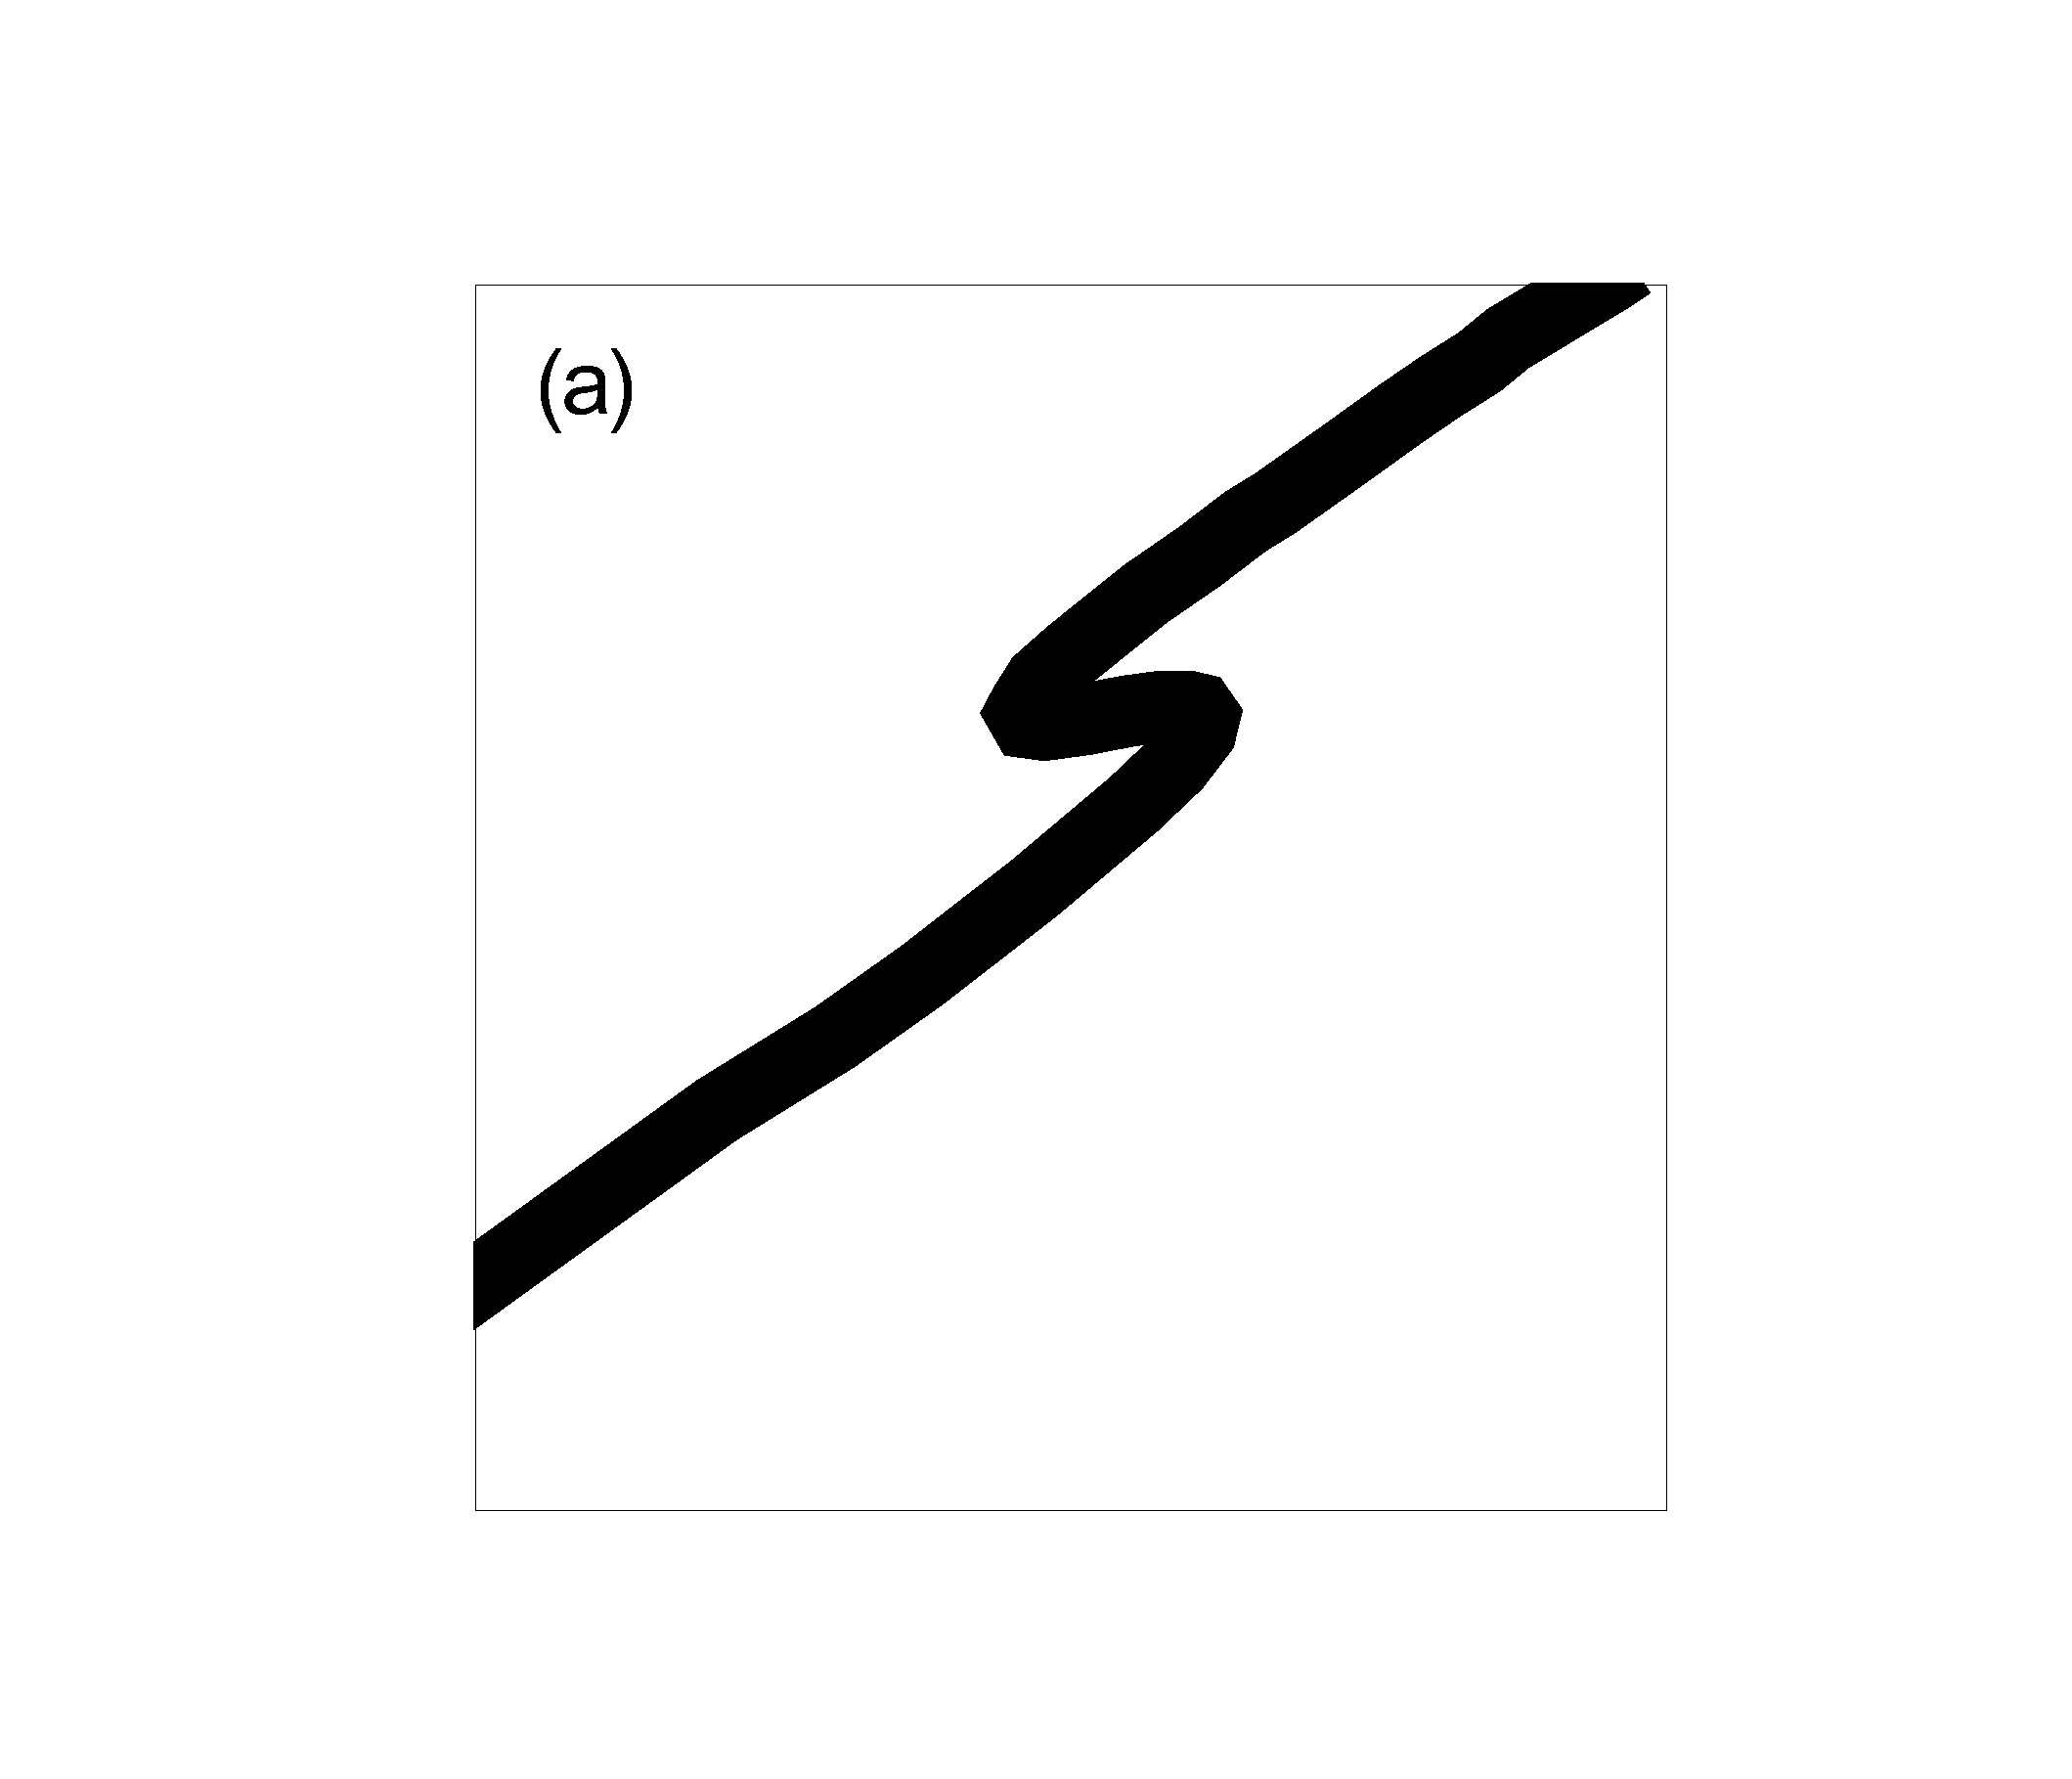
\includegraphics[width=0.9\columnwidth,trim=150 100 150 100,clip]{gfx/aurora_kinked}
	\end{minipage}
	\begin{minipage}{0.3\textwidth}\centering
		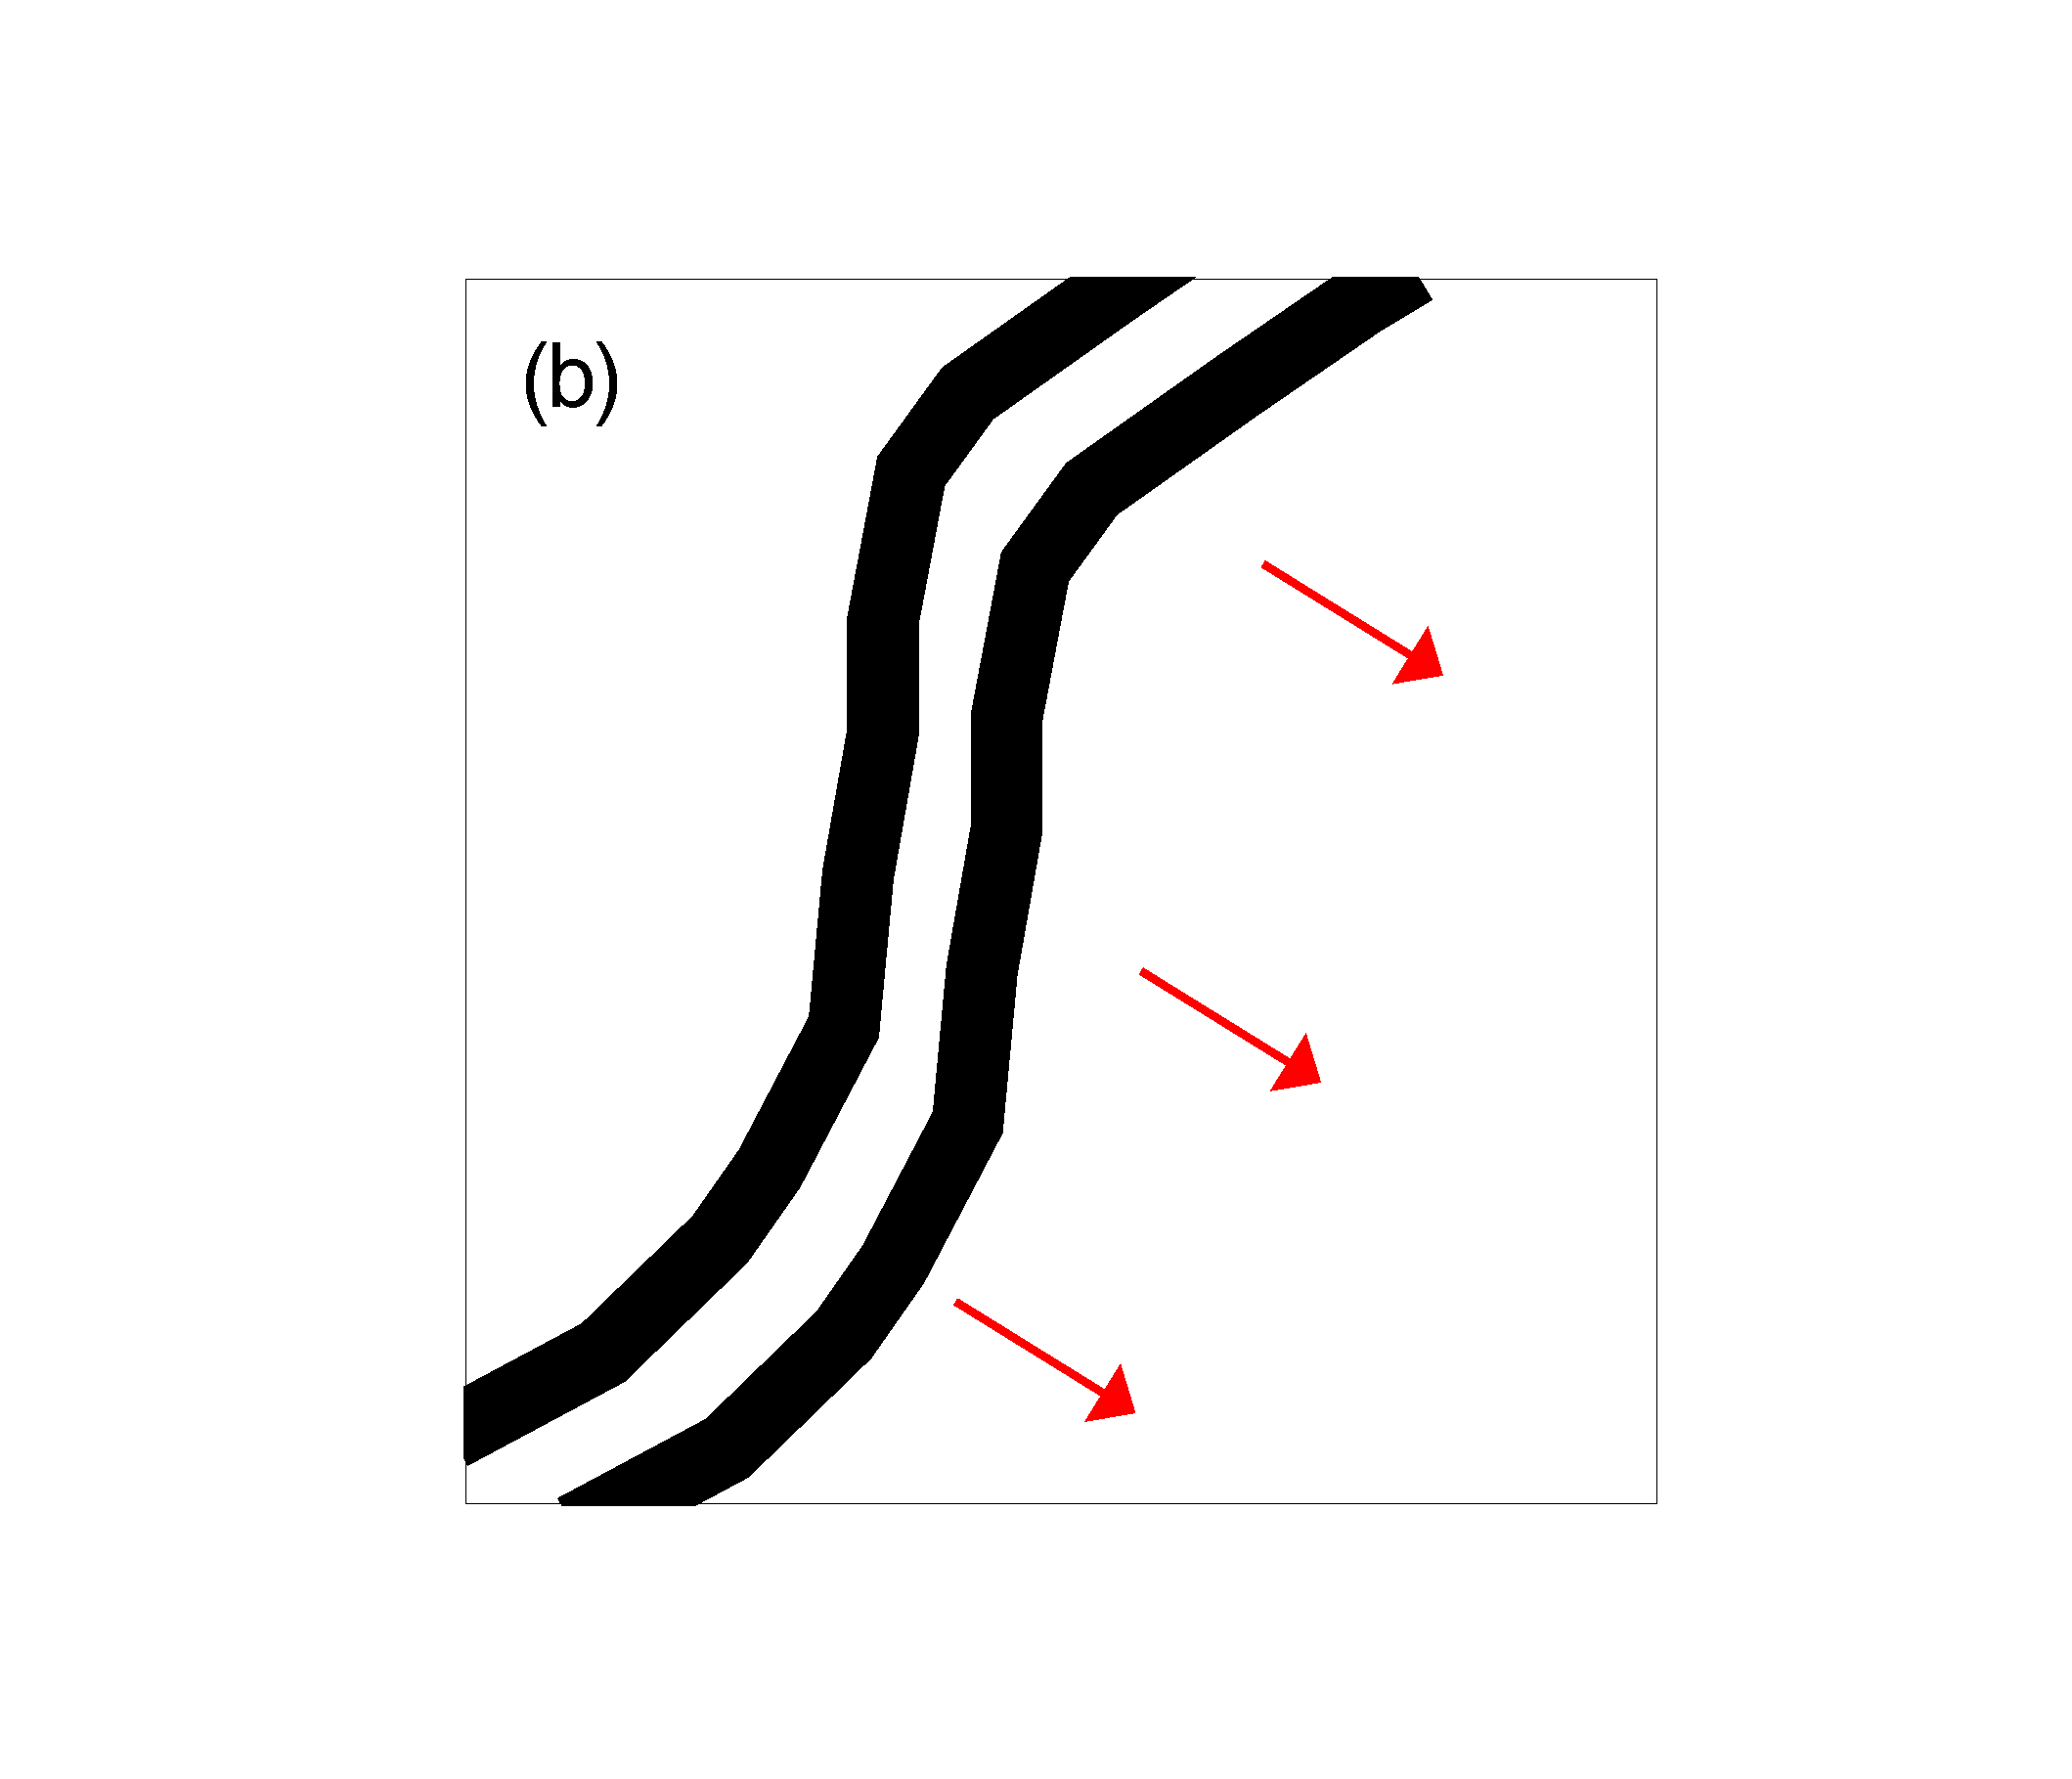
\includegraphics[width=0.9\columnwidth,trim=150 100 150 100,clip]{gfx/aurora_split}
	\end{minipage}
	\begin{minipage}{0.3\textwidth}\centering
		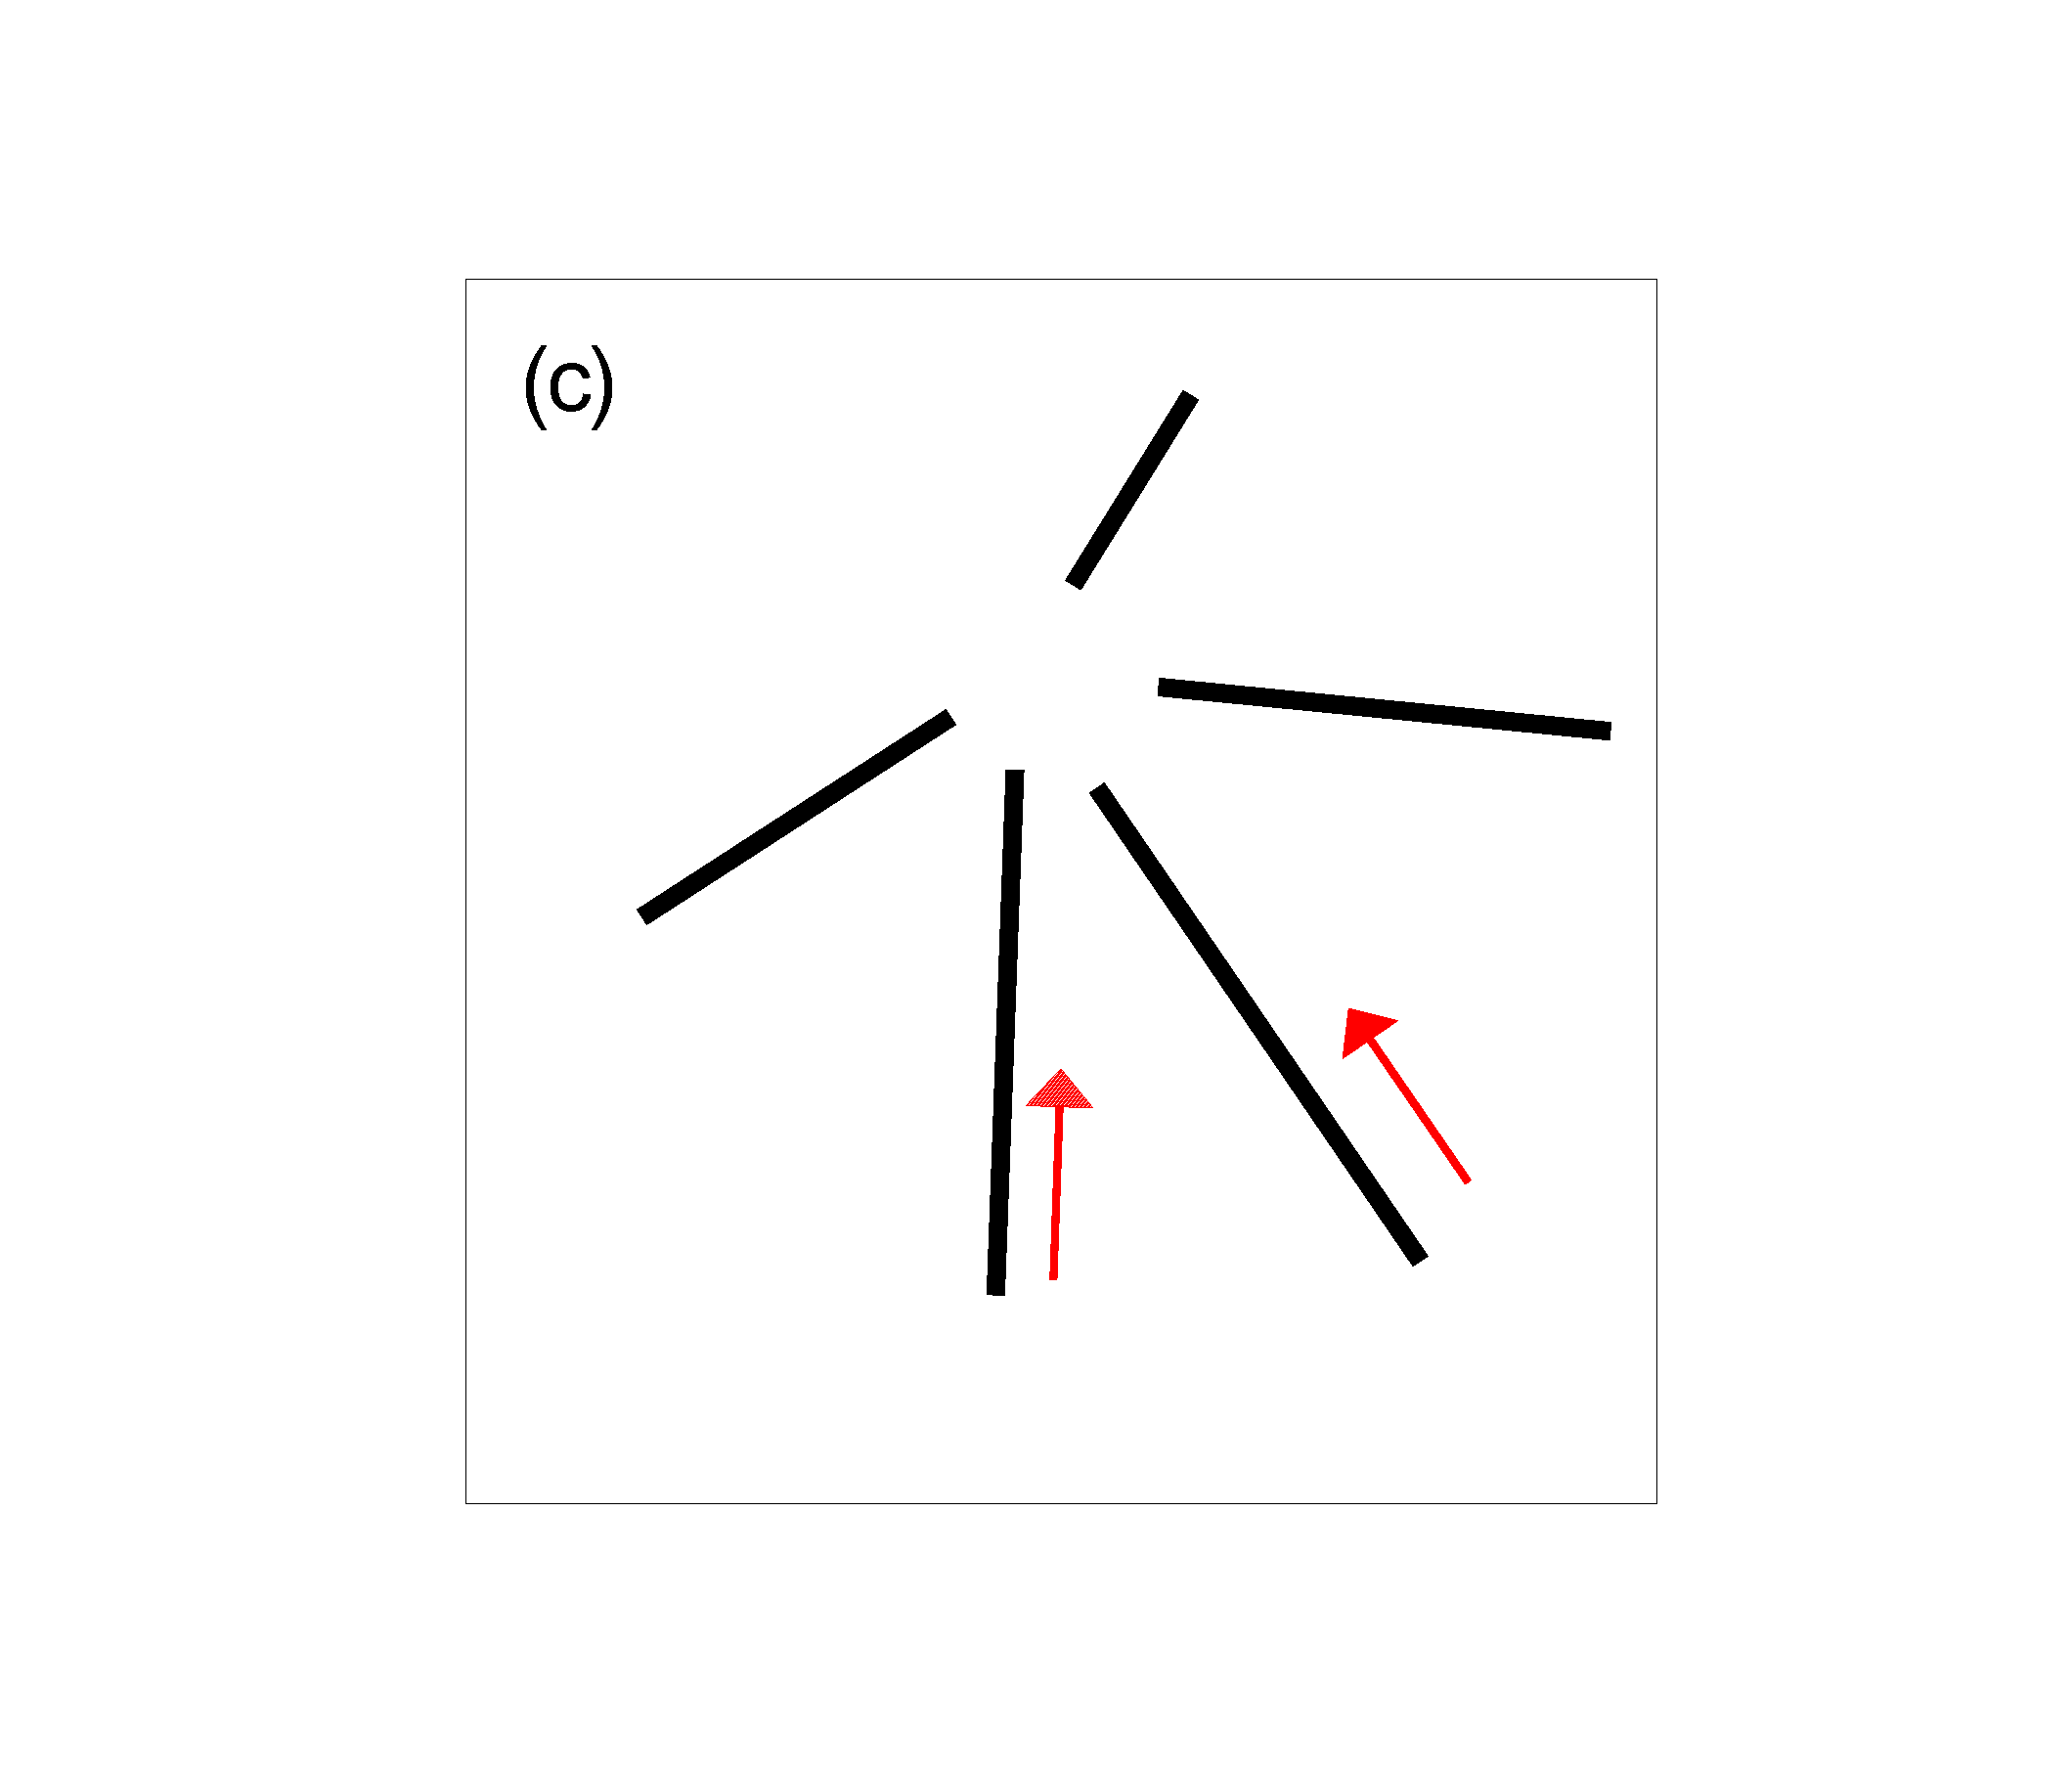
\includegraphics[width=0.9\columnwidth,trim=150 100 150 100,clip]{gfx/aurora_ray}
	\end{minipage}
	\caption{Auroral arc morphologies corresponding to: 
		(a) inverted-V 
		(b) strong Langmuir turbulence 
		(c) streaming upflow}
	\label{fig:cartoonmorph}
\end{figure}
This article presents the first joint analysis of such high-speed, closely spaced multi-camera auroral video using physics model-based iterative reconstruction.
The system is shown to be capable of distinguishing monoenergetic inverted-V electron precipitations (with characteristic energy of several keV) from broadband (tens of eV to several keV) electron precipitations from DAW.
New radar sampling techniques \citep{swoboda2015} enable increasingly fine spatio-temporal resolution suitable for quantifying NEIAL characteristics \citep{schlatter2015}.
ISR measurement cadence of \unit[12]{ms} for ion-line \citep{michell2010} and \unit[200]{ms} for plasma-line \citep{vierinen2016} have been achieved, a factor of 80 improvement over prior plasma-line measurements \citep{nicolls2006}.
Joint optical and ISR measurements targeting NEIALs need to sample faster than \unit[40]{Hz} to capture the temporal dynamics of NEIALs.
Persistent staring automated instruments are required for a practical systems since an entire NEIAL event may last less than half a second \citep{dahlgren2013}.

Joint ISR and high speed filtered optical observations give supporting evidence for apparent connections between DAW aurora and naturally enhanced ion-acoustic lines (NEIALs).
NEIALs are bursty aspect-angle dependent strong ion-line echoes in the lower ionosphere.
Strong echoes in the plasma-line channel accompanied by NEIALs are from Langmuir waves, associated with large fluxes of precipitating electrons \citep{akbari2012}.
The primary electron differential number flux associated with NEIALs has similar sub-second temporal scales and $B_\perp$ scale of \unit[100]{m}.
$B_\perp$ scale width due to anthropogenic heating such as HAARP leads to \unit[100]{m} $B_\perp$ auroral emissions \citep{kelley1995,kendall2010}.
During NEIALs, the ISR fitter algorithms relying upon a Maxwellian ion distribution break down due to non-Maxwellian ion spectrum \citep{knudsen1993}, leading to derived plasma parameters in large error or NaN values.
The mechanisms driving NEIALs are distinct from the electron convection responsible for strong backscatter from Farley-Buneman instabilities arising in the E-region ionosphere below \unit[130]{km} \citep{oppenheim1996,hysell2013}.
Simulation efforts to characterize NEIALs are underway \citep{diaz2008}, but push modern supercomputers such as STAMPEDE to the limits.

\citet{akbari2012} noted open questions on the specific energy transport and deposition processes generating the ionospheric plasma destabilization.
Two possibilities for the energy deposition generating the turbulence are:
\begin{enumerate}
    \item plasma waves intensified directly by primary electron precipitation kinetic processes
    \item plasma waves intensified by secondary suprathermal (hundreds of eV) electrons as a result of the electron beam.
\end{enumerate}
Particle acceleration yielding narrow $B_\perp$ energy flux structure from the magnetosphere into the ionosphere may come from quasi-static electric fields or Alfvén waves.
\citet{akbari2014} speculated that diverse electron precipitation mechanisms may be responsible for driving NEIALs, due to the strong aspect angle dependence of ISR returns.
Rocket observations \citep{knudsen1990} have provided \textit{in situ} measurements distinguishing Alfvén wave accelerated particles from quasi-static accelerated particles.
Since NEIALs may occur for only a few seconds during a substorm, confirmation via \textit{in situ} measurement would take numerous million-dollar rocket launches, each yielding a few minutes of data.
Practical observational means associating Alfvén waves with the turbulence arises from ground-based high speed synchronized cameras used together with ISR.